\section{Evaluation} \label{sec:eval}

Our evaluation was done on a set of three replica machines, with each having 
Linux 3.13.0, 1Gbps bandwidth LAN, 2.80 GHz dual-socket hex-core Intel Xeon 
with 24 hyper-threading cores, 64GB memory, and 1TB SSD.

We evaluated \xxx on \nprog widely used server programs, 
including \http servers \apache~\cite{apache} and \mongoose~\cite{mongoose}; 
\clamav~\cite{clamav}, an anti-virus scanning 
server that scans files in parallel and deletes malicious ones; 
\mediatomb~\cite{mediatomb}, a \upnp multimedia server that uploads, shares, 
and transcodes pictures and videos in parallel; and \mysql~\cite{mysql}, an 
SQL database. Although \mysql has a replication 
feature~\cite{mysql:replication}, this feature is mainly for improving read 
performance, not for providing \smr fault tolerance.

\smr's high availability and fault-tolerance are attractive to these 
servers programs, because these programs provide on-line service and contain 
important in-memory execution states and storage (\eg, \clamav's 
security database, \mediatomb's SQLite~\cite{sqlite} database, and \mysql).

For \apache and \mongoose, we used \apache's own concurrency stress testing 
benchmark \ab to invoke concurrent \http requests for a PHP page, which takes 
about 70 ms for a PHP interpreter to generate the page contents. For \clamav, 
we used its own client utility \v{clamdscan} to request the server to scan 
\clamav's own source code and installation directories in parallel. For 
\mediatomb, because it has a web interface, we used \ab to invoke concurrent 
requests which use \mencoder~\cite{mencoder} to transcode a 15MB video from AVI 
to MP4. For \mysql, we used \sysbench~\cite{sysbench} to generate random select 
queries. These workloads triggered 8$\sim$12 threads in each server program to 
process requests concurrently at peak performance on our machines. These 
popular benchmarks and workloads cover CPU, network, and file-IO 
bounded operations.  

\xxx has two parameters for the \timealgo technique. The first 
parameter, $W_{timeout}$, is the physical duration that the primary's \dmt 
scheduler waits before it requests consensus on a time bubble insertion. To 
prevent this parameter significantly deferring responses, \xxx sets its 
default value 100us, two orders of magnitudes smaller than the workloads' 
response times and wide-area network latencies.

The second parameter, $N_{clock}$, is the number of logical 
clocks within each time bubble. \xxx sets its default value 1000, because we 
observed that the amounts of executed \pthread synchronizations to process each 
request in most of the evaluated servers are closed to this scale. We used 
these default values in all evaluations unless explicitly specified. A 
sensitivity evaluation on these two parameters showed that their default 
values were reasonable choices (\S\ref{sec:sensitivity}).

To mitigate network latency, benchmark clients were ran within 
the replicas' LAN. Larger latency will mask \xxx's overhead. We measured each 
workload's response time as it has direct impact on users. For each data 
point, we ran 1K requests for 20 times and then picked the median value.

The rest of this section focuses on these questions:

\begin{tightenum}

\item[\S\ref{sec:ease-of-use}:] Is \xxx easy to use?

\item[\S\ref{sec:correctness}:] Compared to nondeterministic executions, does 
\xxx consistently enforce the same sequence of network outputs among replicas?

\item[\S\ref{sec:overhead}:] What is \xxx's performance overhead compared to 
nondeterministic executions?

\item[\S\ref{sec:hint}:] When the default schedules enforced by the \parrot 
\dmt scheduler are slow, how much optimization can \parrot's performance hints 
bring to \xxx?

\item[\S\ref{sec:sensitivity}:] How sensitive are the two \timealgo parameters 
to \xxx's performance?

\item[\S\ref{sec:recovery}:] How fast are \xxx's checkpoint and recovery 
components on handling replica failures?


\end{tightenum}







\subsection{Ease of Use} \label{sec:ease-of-use}

All \nprog servers we evaluated were able to be transparently plugged and 
played in \xxx without modification. For \clamav, \mediatomb, and \mysql, we 
did not need to modify any line of code and they already have moderate 
performance overhead compared to the un-replicated nondeterministic executions. 
For \apache and \mongoose, the default schedules serialized parallel 
computations. For each of the two servers, we added two lines of soft barrier 
performance hints invented by \parrot~\cite{parrot:sosp13} to line up parallel 
computations as much as possible and compute efficient \dmt schedules (cf 
\S\ref{sec:hint}).

\subsection{Consistency of Network Outputs} \label{sec:correctness}

To verify whether the server programs running in different replicas maintain 
the same execution states, we compared each server program's network outputs 
logged in three replicas. Network outputs imply a server's execution states, 
including the outcomes of ad-hoc synchronizations and data races, which 
synchronization schedules can not capture. We ran the performance workloads and 
logged the order and contents of server programs' outgoing socket calls, 
including \send, \sendto, \sendmsg, \mywrite, and \pwrite. These calls are 
sufficient to capture all network outputs of the evaluated programs. We then 
used \v{diff} to compare the logs across replicas. 

We designed two experiment plans. In plan I, we ran \xxx with the 
programs. In plan II, we disabled only the \timealgo component in \xxx for 
three reasons: (1) we wanted to know whether \timealgo is needed to keep 
replicas in sync, (2) enabling \paxos made us easy to ship the same workload 
to replicas, and (3) enabling \parrot made us easy to intercepted and logged 
network outputs.

Among the \nprog programs, three server programs, \apache, \mediatomb, 
and \mongoose, used \ab to spawn workloads. In plan I, \xxx's logs from all 
three replicas had the same order and contents of outputs except physical 
times in the responded HTTP headers. In plan II, despite that we disabled only
the \timealgo component, the logs' order of responded HTTP headers and contents 
across replicas were different. Two server programs, \clamav and \mysql, 
used specific benchmarks to spawn workloads. In plan I, the logs showed that 
\xxx enforced the same network outputs. In plan II, the orders of the outputs 
across replicas were different. These experiments suggest that simply combining 
\paxos and \dmt is not sufficient to keep replicas in sync, and the \timealgo 
technique is needed.

To diagnose consistency of network outputs more concisely, we wrote a 
micro-benchmark for \apache. We used the \v{curl} utility to spawn two 
concurrent HTTP requests: a PUT request of a PHP page and a GET request on 
this page, and then we inspected the outcome of the GET request. We ran \apache 
in \xxx with this micro benchmark for 100 times and found that three replicas 
consistently reported the same GET result in each run, either ``200 OK" or 
``404 Not Found", depending on the order of the PUT and GET request arriving at 
the primary's proxy. And then we ran \apache's un-replicated 
execution for 100 times on each replica, and three replicas reported ``404 Not 
Found" for 6, 8, 11 times respectively.

\subsection{Performance Overhead in Normal Case} \label{sec:overhead}

\begin{figure}[t]
\centering
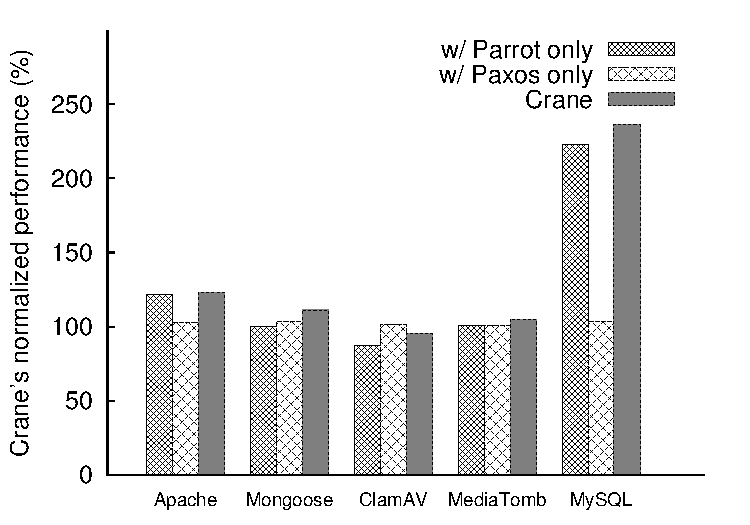
\includegraphics[width=0.5\textwidth]{figures/normalize-perf}
\vspace{-.10in}
\caption{\small {\em \xxx's performance normalized to un-replicated 
nondeterministic execution.}}
\label{fig:normalize-perf}
\end{figure}


To understand the performance impact of \xxx's components, we divided \xxx's 
components into two major parts: the \dmt part ran by \parrot; and the proxy 
(with \paxos) part which enforces the same sequence of client socket 
calls across replicas. Each part ran independently without the other 
part. The proxy part represents the performance overhead of invoking \paxos 
consensus for client socket calls, and the \dmt part represents the \parrot 
\dmt scheduler's overhead.

Figure~\ref{fig:normalize-perf} shows the servers' performance running in 
\xxx normalized by their un-replicated nondeterministic executions. The mean 
overhead of \xxx for the \nprog evaluated programs is \overhead 
due to two main reasons. First, except for \mysql, which does fine-grained, 
per-table mutex and read-write locks frequently, the \dmt schedules were 
efficient on the other four servers. The reason is that \parrot's scheduling 
primitives are already highly optimized for multi-core~\cite{parrot:sosp13}. 
The proxy-only part incurred 0.82\%$\sim$3.46\% overhead, which is not 
surprising, because the number of socket calls is much smaller than 
the number of \pthread synchronizations in these programs. In short, \xxx's 
performance mainly depends on the \dmt schedules' performance.

\mediatomb incurred modest speedup because its transcoder \mencoder had 
significant speedup with \parrot. We inspected \mediatomb's micro performance 
counters with the Intel \vtune~\cite{vtune} profiling tool. When running in 
\xxx, \mediatomb only made 6.6K synchronization context switches, while in the 
\pthread runtime it made 0.9M synchronization context switches. This saving 
caused \mediatomb running with \parrot a 12.76\% speedup compared 
to its nondeterministic execution. The \parrot evaluation~\cite{parrot:sosp13} 
also observed a \mencoderspeedup speedup on the \mencoder program. 

The \timealgo technique saves most of needs on invoking consensus 
for the logical times of clients' socket operations, confirmed by the low 
frequency of inserted time bubbles in Table~\ref{tab:timebubbles}. \apache, 
\mediatomb, and \mongoose uses \ab as its benchmark, and each request contained 
a \connect, \send, and \close call. \clamav uses its own \v{clamdscan} 
benchmark, and each request contained 18 socket calls. \mysql's benchmark 
contained 6$\sim$7 socket calls for each query. The ratio of inserted 
bubbles is merely 6.12\%$\sim$33.35\%. \mediatomb had the highest ratio of time 
bubbles because it took the longest time (9,703ms) to process each 
request.

Note that the number of inserted time bubbles across replicas is the 
same within the same run of \xxx. Within different runs of \xxx, this number 
can be different because \ntimeout is a physical duration.

\begin{table}[b]
\footnotesize
\centering
\vspace{-.05in}
\begin{tabular}{lrrr}
{\bf Program} & {\bf \# client socket calls} & {\bf \# time bubbles}  & {\bf 
\%} \\
\hline\\[-2.3ex]
\apache                       & 3,000        &    450 &    13.04 \\
\clamav                                   & 18,000     &    1,173 &    6.12 \\
\mediatomb                       & 3,000        &    1,501 &    33.35 \\
\mongoose                       & 3,000        &    448 &    12.99 \\
\mysql                       & 6,750        &    573 &    7.82 \\
\end{tabular}
\vspace{-.05in}
\caption{{\em Ratio of time bubbles in all \paxos consensus 
requests.}} 
\label{tab:timebubbles}
\end{table}

\subsection{Optimization of \parrot's Performance Hints} \label{sec:hint}

\begin{figure}[t]
\centering
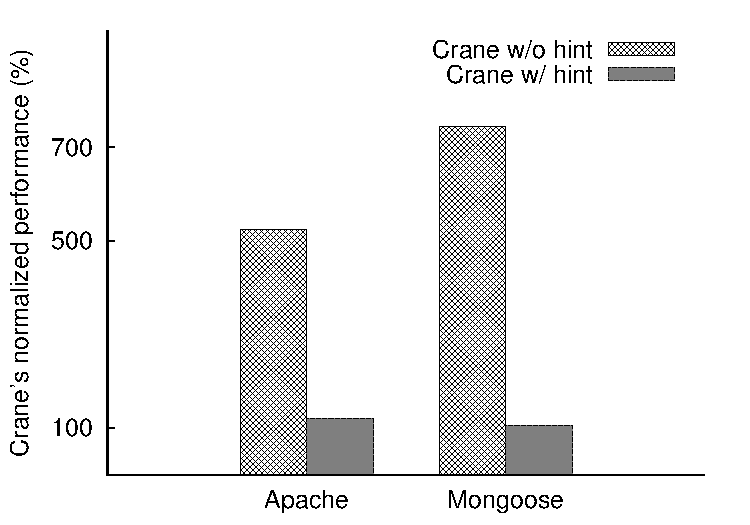
\includegraphics[width=0.5\textwidth]{figures/opt-hint}
\vspace{-.10in}
\caption{\small {Effects of \parrot's soft barrier performance hints.}}
\label{fig:opt-hint}
\end{figure}

In general, a \dmt schedule may be slow in some cases~\cite{parrot:sosp13, 
dthreads:sosp11}, because this schedule may \emph{serialize} some major 
computations that can run in parallel in the \pthread runtime. For instance, 
when we ran \xxx's \dmt scheduler \parrot with \apache and \mongoose, we 
observed that \parrot's default schedules serialized the PHP interpreters.

Fortunately, \parrot creates a set of easy to use, intuitive soft barrier 
hints~\cite{parrot:sosp13} which tell the \dmt runtime to switch to faster 
schedules. These hints are just ``soft" barriers; they timeout 
deterministically and can tolerate different number of concurrent incoming 
requests. They just make a (deterministic) effort to line up computations that 
tend to run in parallel. In addition, these hints can be safely ignored by the 
\parrot runtime without affecting a program's logic.

In our evaluation, we added two lines of hints for each of the \apache and 
\mongoose servers' source code, and the pattern was general: one line was 
added at the server's \v{main()} function to initialize the soft barrier, and 
the other before a PHP interpretation's start to tell the \dmt scheduler 
``these are the major computations to line up". The performance optimization 
effects of these hints are shown in Figure~\ref{fig:opt-hint}. These hints 
reduces \apache's overhead from a 424\% to 22.99\%, and \mongoose's from a 643\% 
to 5.09\%.




\subsection{Sensitivity of Time Bubble Parameters} \label{sec:sensitivity}
\begin{figure}[t]
\centering
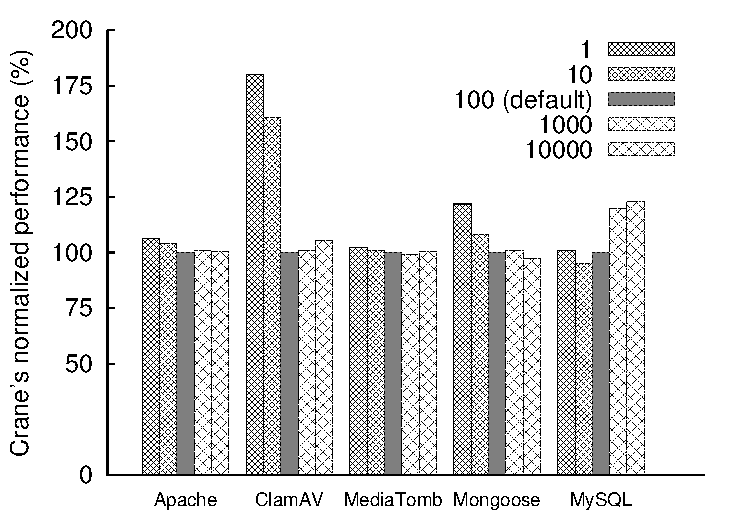
\includegraphics[width=0.5\textwidth]{figures/usleep-sensitivity}
\vspace{-.10in}
\caption{\small {\em \xxx's performance with different settings on \ntimeout 
(us).} Normalized with the default parameter.}
\label{fig:usleep-sensitivity}
\end{figure}

\begin{figure}[t]
\centering
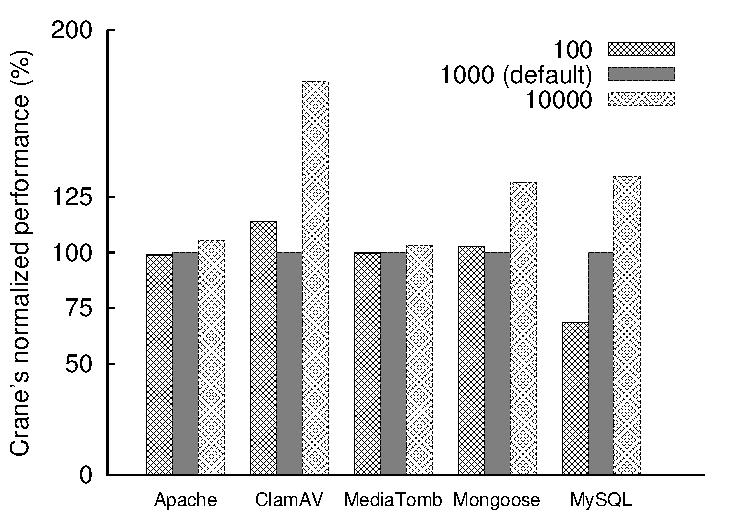
\includegraphics[width=0.5\textwidth]{figures/nclock-sensitivity}
\vspace{-.10in}
\caption{\small {\em \xxx's performance with different settings on \nclock.} 
Normalized with the default parameter.}
\label{fig:nclock-sensitivity}
\end{figure}

The two parameters \ntimeout and \nclock for \timealgo have trade-off on 
performance. This trade-off also depends on each server program as well as its 
performance workload. A smaller \ntimeout means the \dmt 
scheduler can wait less time and then proceed with granted logical clocks with 
inserted time bubbles, but it also means that more time bubbles and thus more 
\paxos consensus are involved. A smaller value also means \timealgo runs 
similar to a per-request consensus approach. 
Figure~\ref{fig:usleep-sensitivity} shows \xxx's performance by only adjusting 
this parameter. \xxx's default setting got the best result for both \apache 
and \clamav, and it got the second best result for the other three programs. 

The \nclock parameter also faces trade-off on performance. A smaller value 
means that servers can exhaust clocks in a time bubble sooner, but if a server 
does lots of \pthread synchronizations to process a request, more time bubbles 
and thus more \paxos consensus are involved. 
Figure~\ref{fig:nclock-sensitivity} shows \xxx's performance by only adjusting 
this parameter. \xxx's default setting got the best result for \clamav, 
\mediatomb, and \mongoose, and the second best result for the other two 
programs.



\subsection{Checkpoint and Recovery} \label{sec:recovery}

\begin{table}[b]
\footnotesize
\centering
\vspace{-.05in}
\begin{tabular}{lrrrr}
{\bf Program} & {\bf C p (ms)} & {\bf R p (ms)} & {\bf C fs (ms)}  & {\bf R fs 
(ms)}\\
\hline\\[-2.3ex]
\apache                       & 33  & 48        &    3,069  & 237 \\
\clamav                               & 415  & 353     &    6,963  & 6,128 \\
\mediatomb                       & 17  & 27        &    2,852  & 213 \\
\mongoose                       & 15  & 31        &    1,294  & 169 \\
\mysql                       & 88  &  81       &    53,473  & 712 \\
\end{tabular}
\vspace{-.05in}
\caption{{\em Average time cost for \xxx's checkpoint and restoring 
component.} ``C p" means ``Checkpoint process", ``R p" means ``Restore 
process", ``C fs" means ``Checkpoint file system", and ``R fs" means 
``Restore file system".} 
\label{tab:checkpoint-time}
\end{table}

To handle replica failures, \xxx periodically invokes a checkpoint operation on 
one backup. Each \xxx checkpoint operation 
contains four time consuming parts: (1) using \criu to dump the state of a 
server process (and its child processes, if any); (2) stopping and restarting a 
\lxc container; (3) doing an incremental checkpoint on a server's current 
working directory and installation directory between the \lxc stop and start; 
and (4) restoring a process's state after the \lxc restart.

Table~\ref{tab:checkpoint-time} shows time costs for each process and file 
system checkpoint operation, and all are median values with 
20 runs. In sum, a process checkpoint or restore took at most 415ms, and a file 
system checkpoint or restore took less than 7s except \mysql. \mysql took about 
one minute to checkpoint its file system because \sysbench generated a large 
database in \mysql's installation directory. For each program, a file system 
restore operation took much less time than its checkpoint operation because a 
restore 
operation patches only files modified by the server program. A common \lxc stop 
and restart operation took 2$\sim$5s depending on the daemon processes' 
bootstrap progress within the container. Although each of these four steps in a 
\xxx checkpoint operation costs time, such a checkpoint is done on only one 
backup replica, its performance impact was negligible in our evaluation (the 
other replicas formed a quorum).

To evaluate the speed of \xxx's \paxos protocol on replica failure and 
recovery, we manually restarted the primary replica running a \mongoose server. 
The other two backups in the system then invoked a leader election with three 
steps~\cite{paxos:practical}, which took \recovertime. After 
the old primary's machine restarted, \xxx restarted the proxy and the 
consensus component, extracted the latest \mongoose checkpoint on the local 
machine and restored the \mongoose process and its file system. On the full 
restore of this \xxx instance, it received the new primary's heart beat message 
in \downgradetime and downgraded itself to a backup. Overall, both the \paxos 
leader election and the restarted old primary's self-downgrading took 
sub-seconds.



